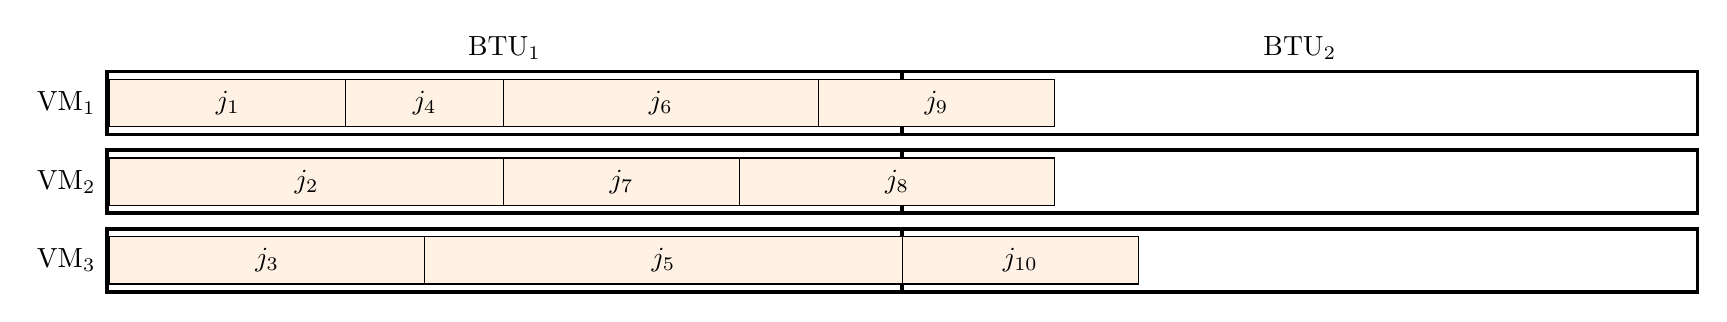
\begin{tikzpicture}[x=10mm,
btu/.style={%
very thick,
minimum height=8mm,
minimum width=101mm,
anchor=west,
draw
},
job/.style={%
anchor=west,
fill=orange!10,
minimum height=6mm,
draw
},
]
%% Line
%%\path[draw,very thick](10.065,-2.5)--(10.065,1);
%%BTUs
\node[btu,label={west:VM$_1$},label={north:BTU$_1$}]at(-0.05,0){};
\node[btu,label={north:BTU$_2$}]at(10.05,0){};
\node[btu,label={west:VM$_2$}]at(-0.05,-1){};
\node[btu]at(10.05,-1){};
\node[btu,label={west:VM$_3$}]at(-0.05,-2){};
\node[btu]at(10.05,-2){};
%%jobs
%\node[job,minimum width=mm]at(,){j};
\node[job,minimum width=30mm]at(0,0){$j_1$};
\node[job,minimum width=50mm]at(0,-1){$j_2$};
\node[job,minimum width=40mm]at(0,-2){$j_3$};
\node[job,minimum width=20mm]at(3,0){$j_4$};
\node[job,minimum width=60.65mm]at(4,-2){$j_5$};
\node[job,minimum width=40mm]at(5,-0){$j_6$};
\node[job,minimum width=30mm]at(5,-1){$j_7$};
\node[job,minimum width=40mm]at(8,-1){$j_8$};
\node[job,minimum width=30mm]at(9,0){$j_9$};
\node[job,minimum width=30mm]at(10.065,-2){$j_{10}$};
\end{tikzpicture}